\documentclass[border=10pt]{standalone}
\usepackage{pgfplots}
\pgfplotsset{compat=1.18}
\begin{document}
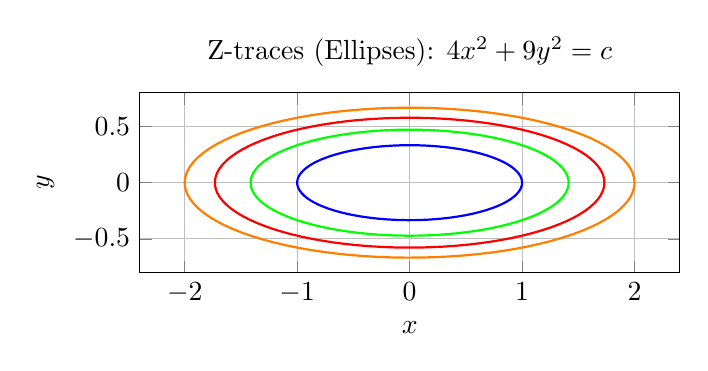
\begin{tikzpicture}
\begin{axis}[
    xlabel=$x$,
    ylabel=$y$,
    title={Z-traces (Ellipses): $4x^2 + 9y^2 = c$},
    grid=major,
    axis equal image,
    ]
    % Draw several ellipses for different z values
    \addplot[domain=0:360, samples=100, thick, blue] ({sqrt(1)*cos(x)}, {sqrt(1/9)*sin(x)});
    \addplot[domain=0:360, samples=100, thick, green] ({sqrt(2)*cos(x)}, {sqrt(2/9)*sin(x)});
    \addplot[domain=0:360, samples=100, thick, red] ({sqrt(3)*cos(x)}, {sqrt(3/9)*sin(x)});
    \addplot[domain=0:360, samples=100, thick, orange] ({sqrt(4)*cos(x)}, {sqrt(4/9)*sin(x)});
\end{axis}
\end{tikzpicture}
\end{document}